%----------------------------------------------------------------------------------------
%	PACKAGES AND DOCUMENT CONFIGURATIONS
%----------------------------------------------------------------------------------------

\documentclass[10pt,a4paper]{article}

% Adjusting margins to personal my need
\addtolength{\oddsidemargin}{-.5in}
\addtolength{\evensidemargin}{-.5in}
\addtolength{\textwidth}{1in}
\addtolength{\topmargin}{-.5in}
\addtolength{\textheight}{1in}

% Graphics
\usepackage{caption}
\usepackage{subcaption}
\usepackage{graphicx}
\graphicspath{{figures/}}

% Math
\usepackage{amssymb}
\usepackage{amsmath} % Required for some math elements 

% Other
\usepackage{algorithmic}
\usepackage{array}
\usepackage{lipsum}
\usepackage{hyperref}
\usepackage{float}




%----------------------------------------------------------------------------------------
%	MAIN PART
%----------------------------------------------------------------------------------------
\begin{document}

\title{Software Quality Assurance Plan (v. 1.0)} % Title
\author{Company 1 - TDDC88}
\date{} % Date for the report
\maketitle % Inserts the title, author and date

\begin{table}
\centering
\begin{tabular}{||c c l c c||} 
\hline
Version & Author & Updates & Reviewed by & Date \\ [0.5ex] 
\hline\hline
0.1 & Erik Sköld & Initial version & - & 2021-09-14 \\
\hline
1.0 & Erik Sköld & 
    \begin{tabular}{@{}l@{}}First plans for documents, \\ development and testing\end{tabular}
    & TBD & 2021-09-23  \\
\hline
\end{tabular}
\end{table}

% Removed abstract, not needed in TDDC88
%----------------------------------------------------------------------------------------
%	Abstract
%----------------------------------------------------------------------------------------
%\begin{abstract}
%\normalsize
%% Text of the abstract
%\lipsum[9]

%\end{abstract}

%----------------------------------------------------------------------------------------
%	Table of Content
%----------------------------------------------------------------------------------------
\setcounter{tocdepth}{2}
\tableofcontents


\clearpage

%----------------------------------------------------------------------------------------
%	Main Part
%----------------------------------------------------------------------------------------
\section{Purpose}
\label{sec:purpose}

The purpose of this Software Quality Assurance Plan is to establish the processes and responsibilities required to implement effective quality assurance functions for the project.

The Software Quality Assurance Plan will provide the framework necessary to ensure a consistent approach to software quality assurance throughout the project life cycle. It defines the approach that will be used by members of the company to monitor and assess software development processes to provide objective insight into the quality of the software and the product. The systematic monitoring of the product and processes will be evaluated to ensure they meet requirements. 

\subsection{Scope}
% This plan covers Software Quality Assurance activities of the project and will be updated regularly.
This plan covers the Software Quality Assurance activities of the project and will be updated regularly.

\subsection{Project description}
% The project's goal is to develop a tool that visualizes and compiles information from patients at Region Östergötland hospital's emergency departments. The information comes from the various computer systems that Region Östergötland has available today. The tool should compile information in an easy and clear way. The compiled information must be presented but does not have to include input solutions.
The project aims to develop a tool that visualizes and compiles information from patients at Region Östergötland hospital's emergency departments. The information comes from the various computer systems that Region Östergötland has available today. The tool should compile information easily and clearly. The compiled information must be presented but does not have to include input solutions.

The product will be developed during four iterations. The project will continue until December 16, 2021, when version 1.0 will be presented.

\subsection{Estimated resources}
\begin{table}[!ht]
\centering
\begin{tabular}{ | l | c |}
    \hline
Task & Estimated hours\\
\hline
Education & 12\\
Developing Quality Processes & 25\\
Documenting Quality Processes & 25\\
Monitor Documents & 14\\
Testing Quality Assurance & 8\\
Software Quality Assessments & 8\\
Supervisor Meetings & 8\\
\hline
\end{tabular}
\end{table}
% \noindent The estimated resources presented in the table above applies for the Quality Coordinator of the project. Education covers both learning about quality assurance and software metrics as well as internal workshops held within the company. Developing Quality Processes and Documenting Quality Processes are the two biggest posts since the company starts from scratch. Work with these tasks is mainly about developing guidelines for the company and documenting them in the Software Quality Assurance Plan and on the company's GitLab. These three posts are the main focus in the first half of the project. More information about Monitoring Documents can be found under subsection \ref{subsec:monitor-docs}, for Testing Quality Assurance see section \ref{sec:testing} and Software Quality Assessments see section \ref{sec:sqa}.
\noindent The estimated resources presented in the table above apply to the project's quality coordinator. Education covers both learning about quality assurance and software metrics as well as internal workshops held within the company. Developing Quality Processes and Documenting Quality Processes are the two biggest posts since the company starts from scratch. Working with these tasks is mainly about developing guidelines for the company and documenting them in the Software Quality Assurance Plan and on the company's GitLab. These three posts are the main focus in the first half of the project. More information about Monitoring Documents can be found under subsection \ref{subsec:monitor-docs}, for Testing Quality Assurance see section \ref{sec:testing} and Software Quality Assessments see section \ref{sec:sqa}.


%\subsection{Quality objectives}
%\textcolor{red}{Develop this! Goals related to testing?}
%\href{https://www.nqa.com/en-gb/resources/blog/may-2016/top-quality-objectives}{https://www.nqa.com/en-gb/resources/blog/may-2016/top-quality-objectives}

%Reach a certain score on SUS-tests, more good comments than bad comments in user testing, improve process..?
\clearpage

\section{Documents}
This section lists the regulatory documents used in the project and the plan for Quality Assurance related to documents.

\subsection{Regulatory documents}
% The Quality Assurance of Documents apply to the six regulatory documents listed below. They are available in the Output documents folder on MS Teams.
The Quality Assurance of Documents applies to the six regulatory documents listed below. They are available in the Output documents folder on MS Teams.

\begin{table}[!ht]
\centering
\begin{tabular}{ | l | l |}
    \hline
Document & Responsible\\
\hline
Architecture Notebook & Jacob Karlén\\
Customer Requirements Specification & Sofie Andersson\\
Education Plan & Axel Nilsson \& Daniel Ma\\
Project Plan & Somaye Gharedaghi \& Axel Nilsson\\
Software Quality Assurance Plan & Erik Sköld\\
Test Plan & Axel Telenius\\
\hline
\end{tabular}
\end{table}

%\begin{itemize}
%\item Architecture Notebook
%\item Customer Requirements Specification
%\item Education Plan
%\item Project Plan
%\item Software Quality Assurance Plan \emph{(this document)}
%\item \textcolor{red}{Standard Operating Procedures}
%\item Test Plan
    %\item User Manual
%\end{itemize}

\subsection{Plan to monitor documents}
\label{subsec:monitor-docs}
% The document guidelines can be found in section 5 of the \href{https://gitlab.liu.se/tddc88-company-1-2021/deploy/-/tree/develop/documents/Project\%20Plan}{Project Plan}. The guidelines cover the process of updating and reviewing the content in the regulatory documents. This procedure is done as an internal inspection before each new published version of a regulatory document to ensure quality. Beside these guidelines, the Quality Coordinator shall monitor the regulatory documents and make sure their structure follow the company guidelines. This will be done every iteration.
The document guidelines can be found in section 5 of the \href{https://gitlab.liu.se/tddc88-company-1-2021/deploy/-/tree/main/documents/Project\%20Plan}{Project Plan}. The guidelines cover the process of updating and reviewing the content in the regulatory documents. This procedure is done as an internal inspection before each newly published version of a regulatory document to ensure quality. Besides these guidelines, the Quality Coordinator shall monitor the regulatory documents and ensure their structure follows the company guidelines. This will be done every iteration.

%The main reviewers for each document will check if the document specific guidelines are followed and if essential content is missing. Remarks from the review is left as comments in the document editor and after the review is over, the reviewer sends a summary of the review to the author of the latest version of the document. This producedure is done as an internal inspection before each new published version of a regulatory document.
%\emph{Lägg till beskrivning och schema över när/hur ofta dokument kommer granskas av Erik? Nej, ingen bra idé :)}
%3/11, 16/11, 30/11, 8/12

%\subsection{Guidelines}
%\emph{For version 1.2 of this document, the guidelines and processes regarding documents is found in the Project Plan (as of 2021-11-04 in section 5 - Processes).} \textcolor{red}{Not published yet!}  
%\begin{itemize}
%\item Regulatory document shall be written in LaTeX, preferably with the help of Overleaf. The documents are made available to everyone in the company through link sharing, editing links to all documents are among the company's files in Teams. 
%\item Version control of the regulatory documents is made via \href{https://gitlab.liu.se/tddc88-company-1-2021/deploy/-/tree/develop}{GitLab}. Each document has its own directory in the documents folder of the develop branch. Version control shall be carried out regularly, at least when each new version of the document is published.
%\item To ensure traceability: When refering to requirements, issues or other artifacts in documentation, ID of the artifact in question must be included. When documenting actions, such as decisions or changes, pointers to relevant documentation must be included.
%\item \textcolor{red}{For major changes to be made to requirements, a change request \emph{(process TBD)} must be accepted by the product owner and reviewed by a company member with knowledge of the subject. Major changes must be documented in accordance with \emph{(process TBD)} where the requirements and issues involved are clearly referred to.}
%\item In order to publish new versions of regulatory documents, a company member with knowledge of the subject must have reviewed the updated document.
%\item When changes are made to published documents, version number, author, significant changes between versions, reviewer and date must be noted in the version table.
%\end{itemize}
\clearpage

\section{Development}
This section is intended to address guidelines for the development and quality assurance of code that will result in the end product.

The project is set up with TypeScript. The client (Angular), server (Node.js) and database (MongoDB) run in three seperate Docker containers and are orchestrated with Docker-compose.

\subsection{Code conventions}
As the project is set up with TypeScript (TS), \href{https://google.github.io/styleguide/tsguide.html}{Google's TypeScript Style Guide} must be followed for all TS code.

Names for functions and variables must be written with camelCase and be self-explanatory. Names generated by Angular should not be changed. \emph{Conventions for HTML and CSS is to be determined}.

\subsection{Workflow}
The project uses a form of feature branch workflow. Feature branches are merged with a development branch, never directly to the main branch. Once the code has passed testing on the develop branch, it can be merged into the main branch by a authorized manager.

\emph{Figure of workflow will be added in an upcoming version.}

\subsection{Software reviews}
In addition to regular discussion of code between developers, software reviews take place in connection with each merge from feature branches to the development branch. The software review must follow a set protocol in GitLab \emph{(will be attached in this docuement in an upcoming version)}. In merge requests, new code must be described as well as what changes have been made and the justification for these.

The reviews are done by a person who has not developed the code himself within two working days of when the merge request was posted. For critical features, the review must be done by a developer with at least competence level 4 \emph{(TBD)}.

\subsection{Bug-tracking system}
GitLab is used for bug-tracking. Bugs will be listed, classified and get unique ID as issues in \href{https://gitlab.liu.se/tddc88-company-1-2021/deploy/-/issues}{the Issues tab of the company GitLab}. \emph{Further guidelines for bug-tracking will be found on the company Gitlab.}

\subsection{Version handling}
GitLab is used for version handling. Work needs to be commited at least daily when working on features but the goal is to commit after each working addition to the code. Commits must be tagged with what kind of commit it is \emph{(see upcoming guidelines on GitLab)} and the commit message should include the ID for the requirement or issue being worked on and the functions that have been changed or added.

\subsection{Documentation}
The Technical Writer and the involved developers document the code produced at module level. The documentation includes descriptions of which inputs are handled, which functions are used, which inputs are given and how they work together with the rest of the system.

\clearpage

\section{Testing}

The Quality Coordinator will assure that the test management processes and products are being implemented per the Test Plan. This includes all types of testing of software system components as described in the test plan, specifically during acceptance testing (validation).

The Quality Coordinator together with the Test Leader will monitor testing efforts to assure that test plans are adhered to and maintained to reflect an accurate progression of the testing activities. It will be assured that tests are conducted using approved test procedures and appropriate test tools, and that test anomalies are identified, documented, addressed, and tracked to closure.

Members of the Test Team will review post-test execution related artifacts including test results and test reports.

\subsection{Purpose}
Testing will be conducted in order to verify that the product is working as intended. Solutions will be evaluated to reduce the risk of problems and improve the performance of the product. Testing is an important part of the work to ensure that the requirements are complied with and thus assuring quality.

\subsection{Test plan}
The latest published version of the Testplan is available in the Output folder on MS Teams and on \href{https://gitlab.liu.se/tddc88-company-1-2021/deploy/-/tree/develop/documents/Test\%20Plan}{GitLab}. The test tools used are different features on GitLab (automatic test pipeline in merge requests, bug tracking with the help of issues and comments), Karma and Selenium. If bugs are found during system and acceptance testing, they are reported using comments and issues in GitLab. Test results from CTA and SUS testing are recorded and noted in a document template for each test. The results are summarized and feedback from the users are forwarded to developers and UX-designers.  

%\bigskip
%\noindent \textcolor{red}{Need to include links to testing documentation, specify what tools are used for testing and how test results are reported. A plan for assuring quality for the test cases...}

\subsection{Quality assurance with test cases}
To avoid biased testing and a limited coverage, the test plan and test cases are written and developed by designated testers who have not worked with the code that is to be tested. Every test case shall have a clear objective, for example focus on one feature at the time. The test case is broken down into a series of concise steps and when an action is taken, the tester or an automated test should be able to easily measure the success of the action. To ensure meeting expectations from the intended end-user, the acceptance testing is primarily made with medical personnel.
\clearpage

\section{Software Quality Assessments}
This section describes the plan for Software Quality Assessments (excluding testing). The plan includes a schedule of the assessments, their purpose and the metrics to be used.

%highlights the expected resources to be spent on Quality Assurance (excluding testing) and the standard metrics to be used. \emph{Will be further developed in a future version.}

%   Removed to version 1.2
%\subsection{Resources \textcolor{red}{(UPDATE OR REMOVE)}}
%\begin{table}[H]
%\centering
%\begin{tabular}{||c c||} 
%\hline
%Quality Personnel & Hours \\ [0.5ex] 
%\hline\hline
%Quality Coordinator & 80 \\
%\hline
%\end{tabular}
%\end{table}

\subsection{Assessment schedule}
\begin{table}[H]
\centering
\begin{tabular}{||c c||} 
\hline
Date & Iteration to be monitored \\ [0.5ex] 
\hline\hline
2021-11-09 & Work until iteration 2 \\
\hline
2021-11-29 & Iteration 3 \\
\hline
2021-12-07 & Iteration 4 \\
\hline
\end{tabular}
\end{table}

\subsection{Purpose of assessments}
The purpose of this procedure is to monitor and measure the product quality. Data is collected to find risks and determine if changes in the product or processes are needed.

%\begin{itemize}
%    \item Plan quality assurance (Gör en plan för hur ofta och vad som ska göras, hur ska det rapporteras? Baserat på detta kan metrics avgöras.)
%    \item Monitor and measure product quality
%    \item Initiates necessary changes of product and processes
%    \item Review decisions on code condventions, test tools and reporting
%    \item Collect means of quality work
%    \item Use CodeMR for software metrics? Complexity, Coupling, Lack of Cohesion, Size
%\end{itemize}

\subsection{Metrics}
For each assessment, the Quality Coordinator will measure and produce the metrics listed below. The results shall be documented in a spreadsheet available to the entire company in MS Teams. A summary of the assessment will be placed in the Output folder on MS Teams. The most significant findings will be brought up at the weekly manager meeting by the Quality Coordinator, where a decision is made whether any further action needs to be taken.

\subsubsection{Quality of code}
%\subsubsection{CodeMR}
\begin{itemize}
%    \item Complexity
%    \item Coupling
%    \item Lack of Cohesion
%    \item Size
\item Ratio of comments per function
\item Ratio of commit messages following the company guidelines
\item Number of files and directories within server and client respectively
\end{itemize}
These metrics are noted manually and will indicate the quality of the code with regards to maintainability and understandability.
%These metrics are given from the code analysis tool CodeMR. The metrics will give an overview of which classes have for example high complexity. If certain classes have too high values, this will be noticed and remedied. The goal is that no class should have a high or very-high value of these quality attributes.

\subsubsection{GitLab}
\begin{itemize}
    \item Deployment frequency (Planned vs Actual)
    \item WIP amount (amount of "cards" or tasks in progress at the time)
    \item Number of Peer Reviews (reviewed Merge Requests)
    \item Ratio of merges without review
    \item Time to merge (time from first commit to merge request sent)
    \item Merge request review time
    \item Number of Issues found when reviewing Merge requests
\end{itemize}
These metrics are produced from the activities on the company GitLab. The purpose of them is to monitor and evaluate the processes and workflow on GitLab. If the metrics show values worse than the set guidelines, actions will be taken to meet the guidelines.

\subsubsection{Quality process}
\begin{itemize}    
    \item Number of Software Quality Assessments (Planned versus Actual)
    \item Number of Software Quality Assessment Findings (Open versus Closed)
    \item Number of Risks identified as a result of Software Quality Assessments
\end{itemize}
The purpose of these metrics is to evaluate the Software Quality Assessments. The values of these metrics will indicate how rewarding the process is.
\clearpage


%----------------------------------------------------------------------------------------
%	Appendix
%----------------------------------------------------------------------------------------
%% \newpage
\appendix

\section{Development process}
\label{sec:dev-process-appendix}
 \begin{figure}[h!]
     \centering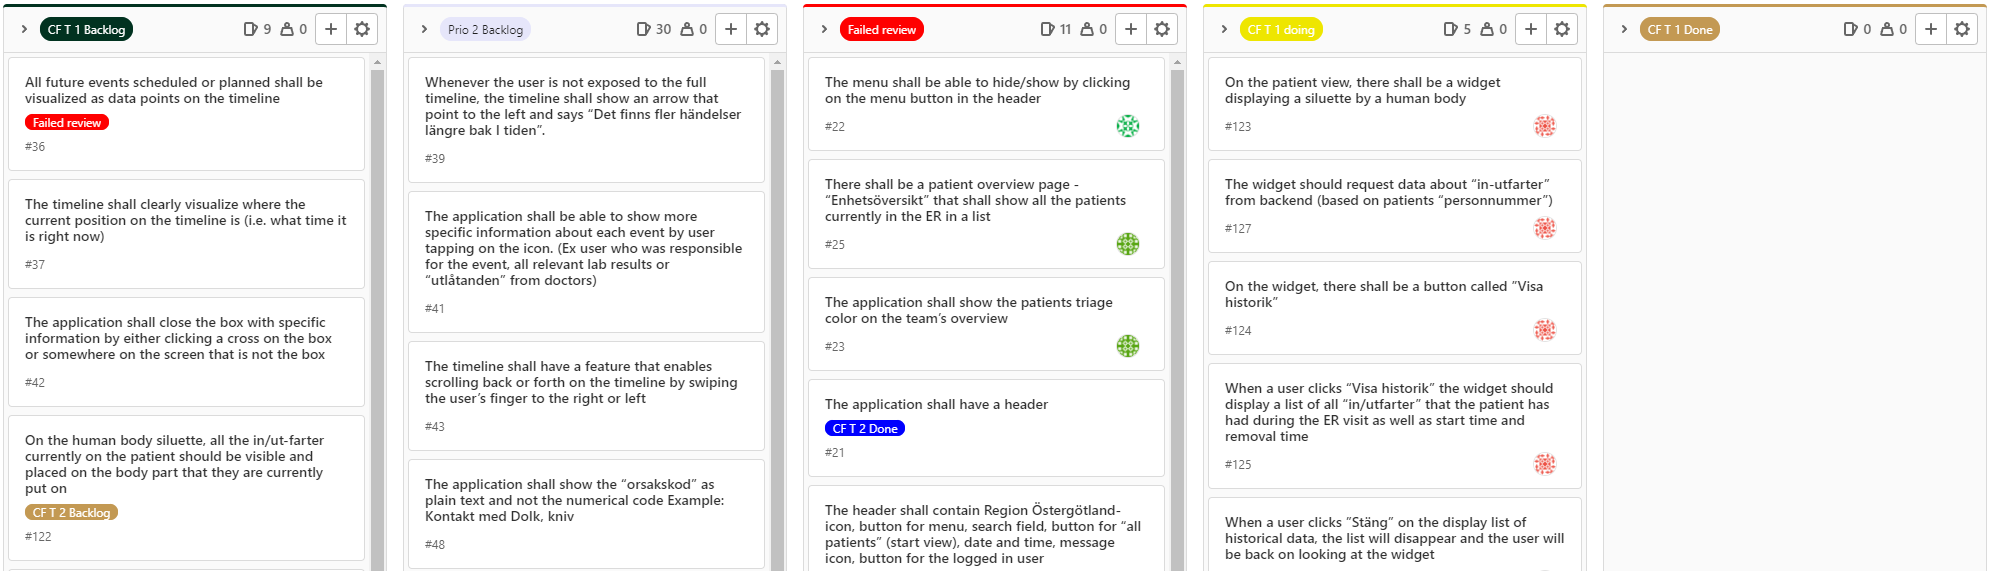
\includegraphics[width=1 \linewidth]{figures/Gitlab board.PNG}
     \caption{GitLab Board}
     %\label{appendix: gitlabboard}
\end{figure}

% Currently no need for appendix

%----------------------------------------------------------------------------------------
%	Bibliography
%----------------------------------------------------------------------------------------
%\clearpage
%\bibliography{bibliography/sample}{}
%\bibliographystyle{plain}

\end{document}